%\addcontentsline{toc}{chapter}{Development Process}
\chapter{Design \& Implementation}

The structure of this chapter follows the agile methodology used to develop the
Quiz Tool. Each section contains information about a sprint, allowing the reader
to gain more understanding of how the design and the tool itself evolved over time.

\section{Sprint 1 - Hello Quiz Tool}
\subsection{Sprint Planning}
The first sprint of the Quiz Tool focused on setting up the DevOps of the project,
and deployment of a "hello world" version of the tool consisting of the front end,
back end and nginx\cite{34} running together using docker-compose. It was also important
to investigate how to best structure the application to include both the front and the
back end of the application in a single GitHub repository. The following subsections
cover the most important aspects of the sprint, and the entire list of estimated
stories can be found in the \autoref{chap:spintstories} of this report.

\subsection{Application Structure}
The main goal of using docker-compose, was to have the whole application running in
the same manner locally on the developer's machine, during testing on Circle CI, and
in the production environment. This meant the application had to be containerised
using Docker, and containers had to be able to communicate with each other appropriately.
This was even more difficult considering Socket.io had to be incorporated, to allow
real time broadcast of lecture slides to students in the future. I have decided to
create a prototype of a very basic chat application, containerised using Docker and
orchestrated using docker-compose. The prototype had to be written in the MEAN stack,
and use Socket.io to prove it was possible to make all technologies work together.

\begin{figure}[ht]
    \centering
    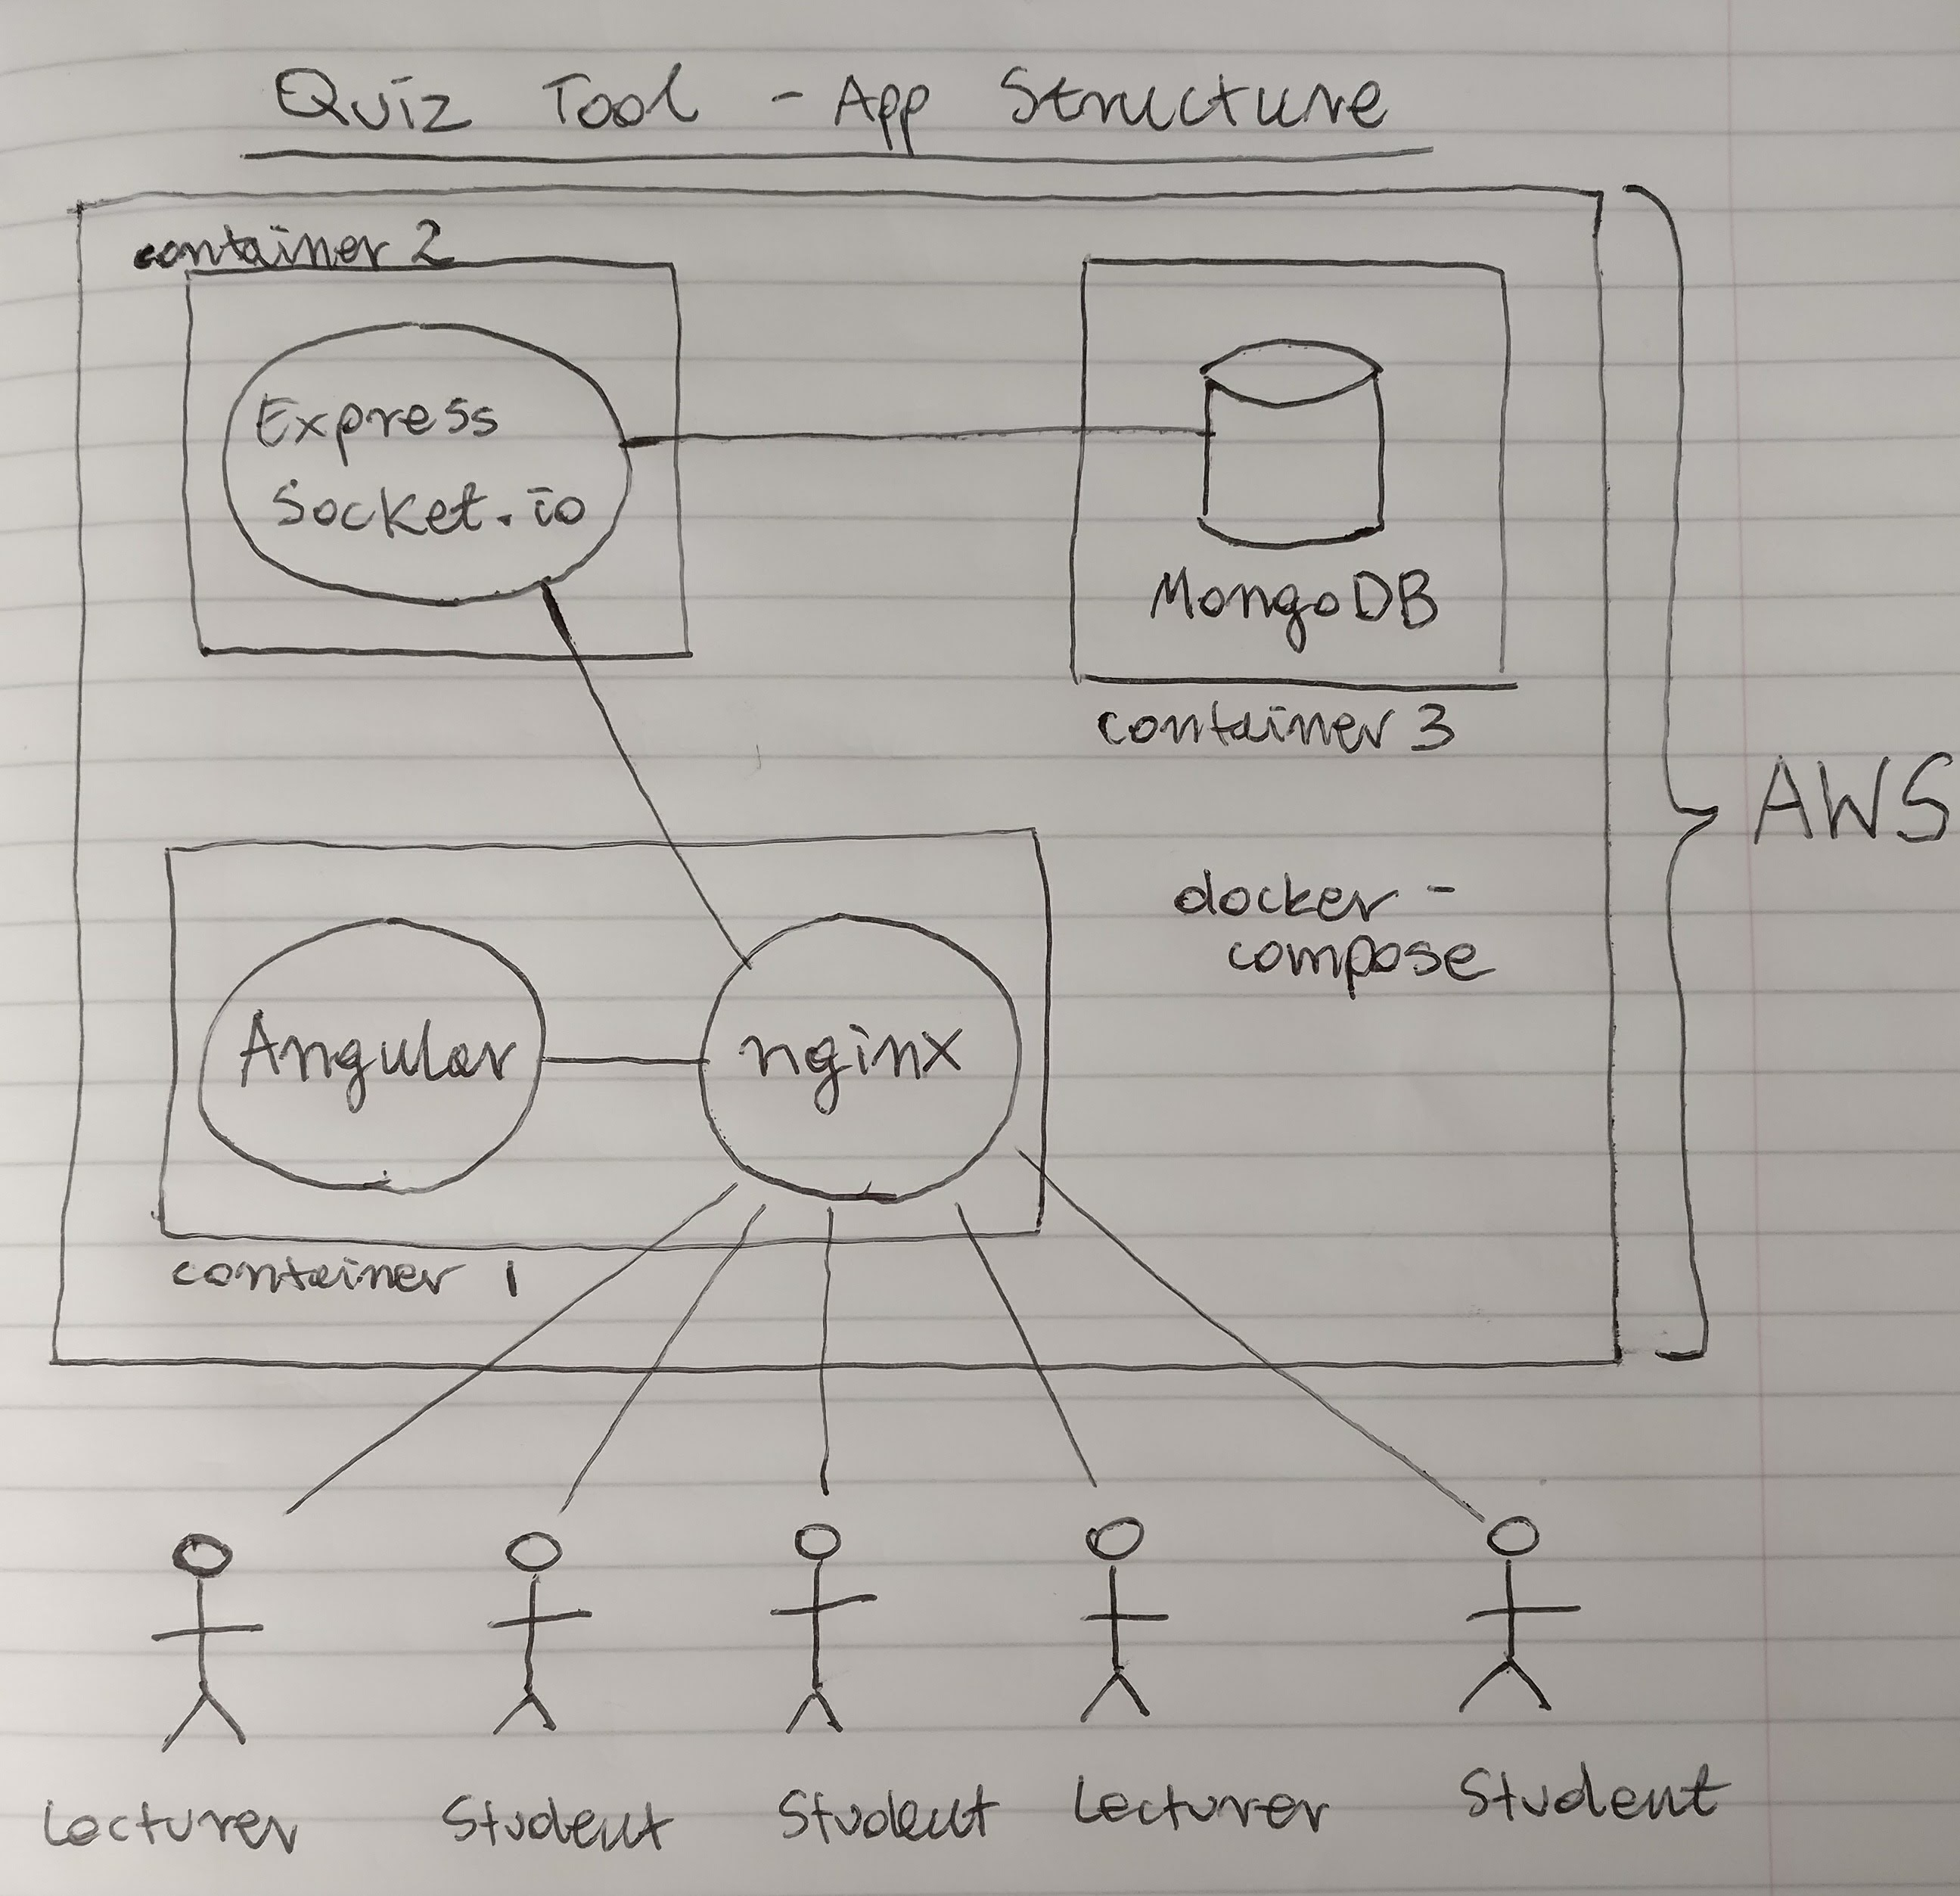
\includegraphics[width=0.7\textwidth]{../../design/app_structure.jpg}
    \caption{The proof of concept application structure}
    \label{fig:appstrucure}
\end{figure}

\subsection{Continuous Integration}

\subsection{Production Environment}

\subsection{Story Boards}

\subsection{Sprint Retrospective}

\section{Sprint 2 - Bare Bone Application}
\subsection{Sprint Planning}

\subsection{Sprint Retrospective}
\section{Sprint 3 - Add Quizes}
\subsection{Sprint Planning}

\subsection{Sprint Retrospective}
\section{Sprint 4 - Fancy Quizes and Defect Fixing}
\subsection{Sprint Planning}

\subsection{Sprint Retrospective}
\section{Sprint 5 - Persistence, Report Generation and Testing}
\subsection{Sprint Planning}

\subsection{Sprint Retrospective}

\chapter{Final Design}

This chapter follows on the discussion of the individual sprints and summarises
the final design of the tool.

\chapter{Testing}

\section{Server Side Unit Tests}
\section{Client Side Unit Tests}
\section{Selenium Integration Tests}

% You should concentrate on the more important aspects of the design. It is essential that an overview is presented before going into detail. As well as describing the design adopted it must also explain what other designs were considered and why they were rejected.
%
% The design should describe what you expected to do, and might also explain areas that you had to revise after some investigation.
%
% Typically, for an object-oriented design, the discussion will focus on the choice of objects and classes and the allocation of methods to classes. The use made of reusable components should be described and their source referenced. Particularly important decisions concerning data structures usually affect the architecture of a system and so should be described here.
%
% How much material you include on detailed design and implementation will depend very much on the nature of the project. It should not be padded out. Think about the significant aspects of your system. For example, describe the design of the user interface if it is a critical aspect of your system, or provide detail about methods and data structures that are not trivial. Do not spend time on long lists of trivial items and repetitive descriptions. If in doubt about what is appropriate, speak to your supervisor.
%
% You should also identify any support tools that you used. You should discuss your choice of implementation tools - programming language, compilers, database management system, program development environment, etc.
%
% Some example sub-sections may be as follows, but the specific sections are for you to define.

% \section{Overall Architecture}
%
% \section{Some detailed design}
%
% \subsection{Even more detail}
%
% \section{User Interface}
%
% \section{Other relevant sections}

% \chapter{Implementation}
% The implementation should look at any issues you encountered as you tried to implement your
% design. During the work, you might have found that elements of your design were unnecessary or
% overly complex; perhaps third party libraries were available that simplified some of the functions
% that you intended to implement. If things were easier in some areas, then how did you adapt your
% project to take account of your findings?
% It is more likely that things were more complex than you first thought. In particular, were there
% any problems or difficulties that you found during implementation that you had to address? Did
% such problems simply delay you or were they more significant?
% You can conclude this section by reviewing the end of the implementation stage against the
% planned requirements

% \chapter{Testing}
%
% Detailed descriptions of every test case are definitely not what is required here. What is important is to show that you adopted a sensible strategy that was, in principle, capable of testing the system adequately even if you did not have the time to test the system fully.
%
% Provide information in the body of your report and the appendix to explain the testing that has been performed. How does this testing address the requirements and design for the project?
%
% How comprehensive is the testing within the constraints of the project?  Are you testing the normal working behaviour? Are you testing the exceptional behaviour, e.g. error conditions? Are you testing security issues if they are relevant for your project?
%
% Have you tested your system on ``real users''? For example, if your system is supposed to solve a problem for a business, then it would be appropriate to present your approach to involve the users in the testing process and to record the results that you obtained. Depending on the level of detail, it is likely that you would put any detailed results in an appendix.
%
% The following sections indicate some areas you might include. Other sections may be more appropriate to your project.

% \section{Overall Approach to Testing}
%
% \section{Automated Testing}
%
% \subsection{Unit Tests}
%
% \subsection{User Interface Testing}
%
% \subsection{Stress Testing}
%
% \subsection{Other types of testing}
%
% \section{Integration Testing}
%
% \section{User Testing}
